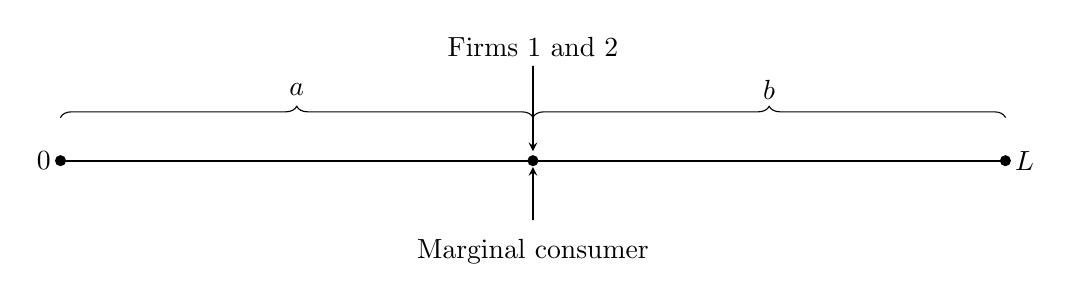
\begin{tikzpicture}[>=stealth, line cap=round]
\def\xO{0}
\def\xM{6}   % marginal consumer / co-location point of firms 1 and 2
\def\xL{12}
\draw[thick] (\xO,0) -- (\xL,0);
\fill (\xO,0) circle (2pt);
\fill (\xM,0) circle (2pt);
\fill (\xL,0) circle (2pt);
\node[left]  at (\xO,0) {$0$};
\node[right] at (\xL,0) {$L$};
\draw[decorate, decoration={brace, amplitude=4pt}]
  (\xO,0.55) -- (\xM,0.55) node[midway, yshift=10pt] {$a$};
\draw[decorate, decoration={brace, amplitude=4pt}]
  (\xM,0.55) -- (\xL,0.55) node[midway, yshift=10pt] {$b$};
\node at (\xM,1.45) {Firms 1 and 2};
\draw[->] (\xM,1.20) -- (\xM,0.12);
\node[align=center] at (\xM,-1.15) {Marginal consumer};
\draw[->] (\xM,-0.75) -- (\xM,-0.08);
\end{tikzpicture}